\documentclass[aspectratio=169]{beamer}
\usepackage[utf8]{inputenc}

\usepackage{graphicx}
\graphicspath{{"C:/Users/caleb/OneDrive - University of North Carolina at Chapel Hill/Documents/HPV MultiSexID/multiSexID_pack/plots/"}}
\setbeamertemplate{caption}{\raggedright\insertcaption\par}
\setbeamertemplate{navigation symbols}{}
\setbeamertemplate{bibliography item}[text]
\usefonttheme{professionalfonts}
\usefonttheme{serif}
\usetheme{Pittsburgh}
\usecolortheme{seahorse}
\usepackage{color}
\definecolor{mygray}{gray}{0.6}

\usepackage{booktabs}
\usepackage{amssymb}
\usepackage{amsmath}
\usepackage{amsthm}
\usepackage{wrapfig}
\usepackage{adjustbox}
\renewcommand*{\thefootnote}{\fnsymbol{footnote}}

% \usepackage[style = authoryear, backend = biber, doi = false, url = false, maxbibnames = 5]{biblatex}
% remove notes: from http://tex.stackexchange.com/questions/208441/suppress-the-note-field-using-biblatex
%\AtEveryBibitem{%
 %\clearfield{note}%
  %\clearfield{issn}%
%}

%\renewcommand*{\bibfont}{\scriptsize}
%\bibliography{smdm2018}

\title{\textbf{Beyond Hetero}}
\subtitle{The Impact of Disregarding Non-Heterosexual Partnerships in Mathematical Models of Human Papillomavirus}
\author[Caleb Easterly]{\textbf{Caleb Easterly\inst{1}}, Fernando Alarid-Escudero, PhD\inst{1}, \\ Shalini Kulasingam, PhD\inst{2}, Eva Enns, PhD\inst{1}}
\date{\today}
\institute
{
  \inst{1}%
  Division of Health Policy and Management\\University of Minnesota School of Public Health
  \and
  \vskip-2mm
  \inst{2}%
  Division of Epidemiology\\University of Minnesota School of Public Health
}

% from http://tex.stackexchange.com/questions/178800/creating-sections-each-with-title-pages-in-beamers-slides
\AtBeginSection[]{
  \begin{frame}
  \vfill
  \centering
  \begin{beamercolorbox}[sep=8pt,center,shadow=true,rounded=true]{title}
    \usebeamerfont{title}\insertsectionhead\par%
  \end{beamercolorbox}
  \vfill
  \end{frame}
}


\begin{document}


\begin{frame}
\titlepage
\end{frame}

% 
% \begin{frame}{Research Question}
% \begin{itemize}
% \item 
% \end{itemize}
% How do the benefits of human papillomavirus (HPV) vaccination of men predicted by a multiple sexual identity model compare to those predicted by a heterosexual-only model?
% \end{frame}

\begin{frame}{Epidemiology of HPV}
    \begin{columns}[T]
        \begin{column}{0.5\textwidth}
            \begin{itemize}
                \pause
                \item HPV is the most common sexually transmitted infection (STI), and is common in people of all sexual identities
                \pause
                \item Vaccines can effectively prevent much high-risk HPV infection
                \pause
                \item High-risk HPV causes cancer at several anatomical sites
            \end{itemize}
        \end{column}
        \begin{column}{0.4\textwidth}
            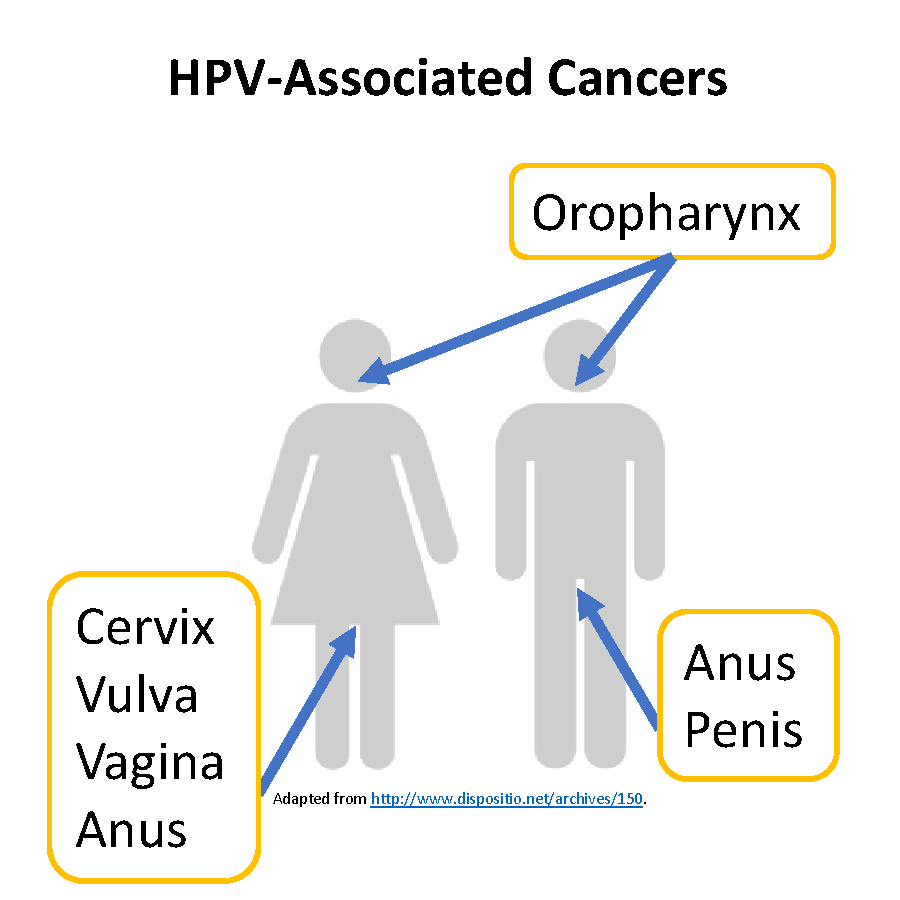
\includegraphics[width=\textwidth]{hpv_cancers.pdf}
        \end{column}
    \end{columns}
\end{frame}

\begin{frame}{Modeling of HPV}
    \begin{itemize}
        \item Transmission modeling of human papillomavirus (HPV)  vaccination is used to evaluate and compare vaccination policies
        \pause
        \item The vast majority of HPV models only consider a heterosexual population
        \pause
        \item These models are used to determine vaccination policy for people of all sexual identities
        \pause
        \item In 2017, the interim statement of the UK Joint Committee on Vaccination and Immunisation recommended against vaccinating boys, based on cost-effectiveness estimates from:
        \pause
        \begin{itemize}
            \item a heterosexual-only model (Public Health England)
            \pause
            \item a meta-analysis of 16 heterosexual-only models (Brisson, et al., 2016)
            \pause
            \item a model from the University of Warwick (unpublished) \pause
            \item other evidence
        \end{itemize}
    \end{itemize}
\end{frame}






\begin{frame}{Why go beyond hetero?}
\begin{columns}
    \begin{column}{0.5\textwidth}
        \begin{itemize}
            \item More representative \pause
            \item A seat at the policy-making table (justice, equity) \pause
            \item Identify disparities in benefit \pause
            \item Match population to calibration targets
        \end{itemize}
    \end{column}
    \begin{column}{0.5\textwidth}
        \begin{figure}
            \framebox{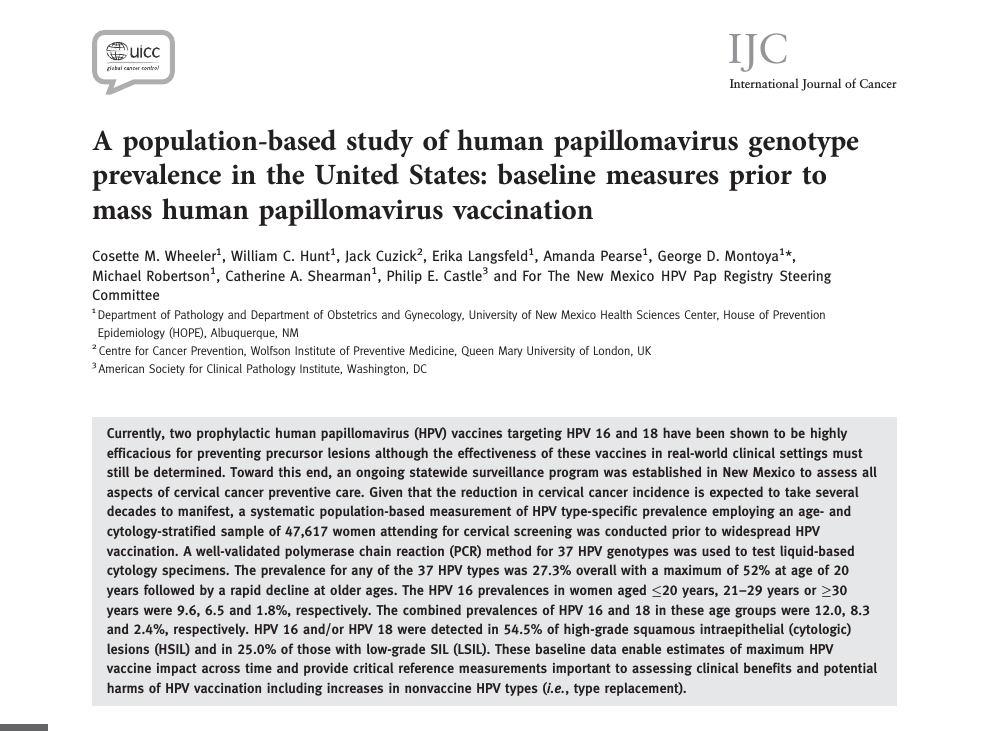
\includegraphics[width=\textwidth]{wheeler_2013}}
            \caption{Wheeler, et al. 2013}
        \end{figure}
    \end{column}
\end{columns}
\end{frame}


\begin{frame}{Model Details}
    \begin{columns}[T]
    \begin{column}{0.5\textwidth}
        \centering
        \begin{figure}
            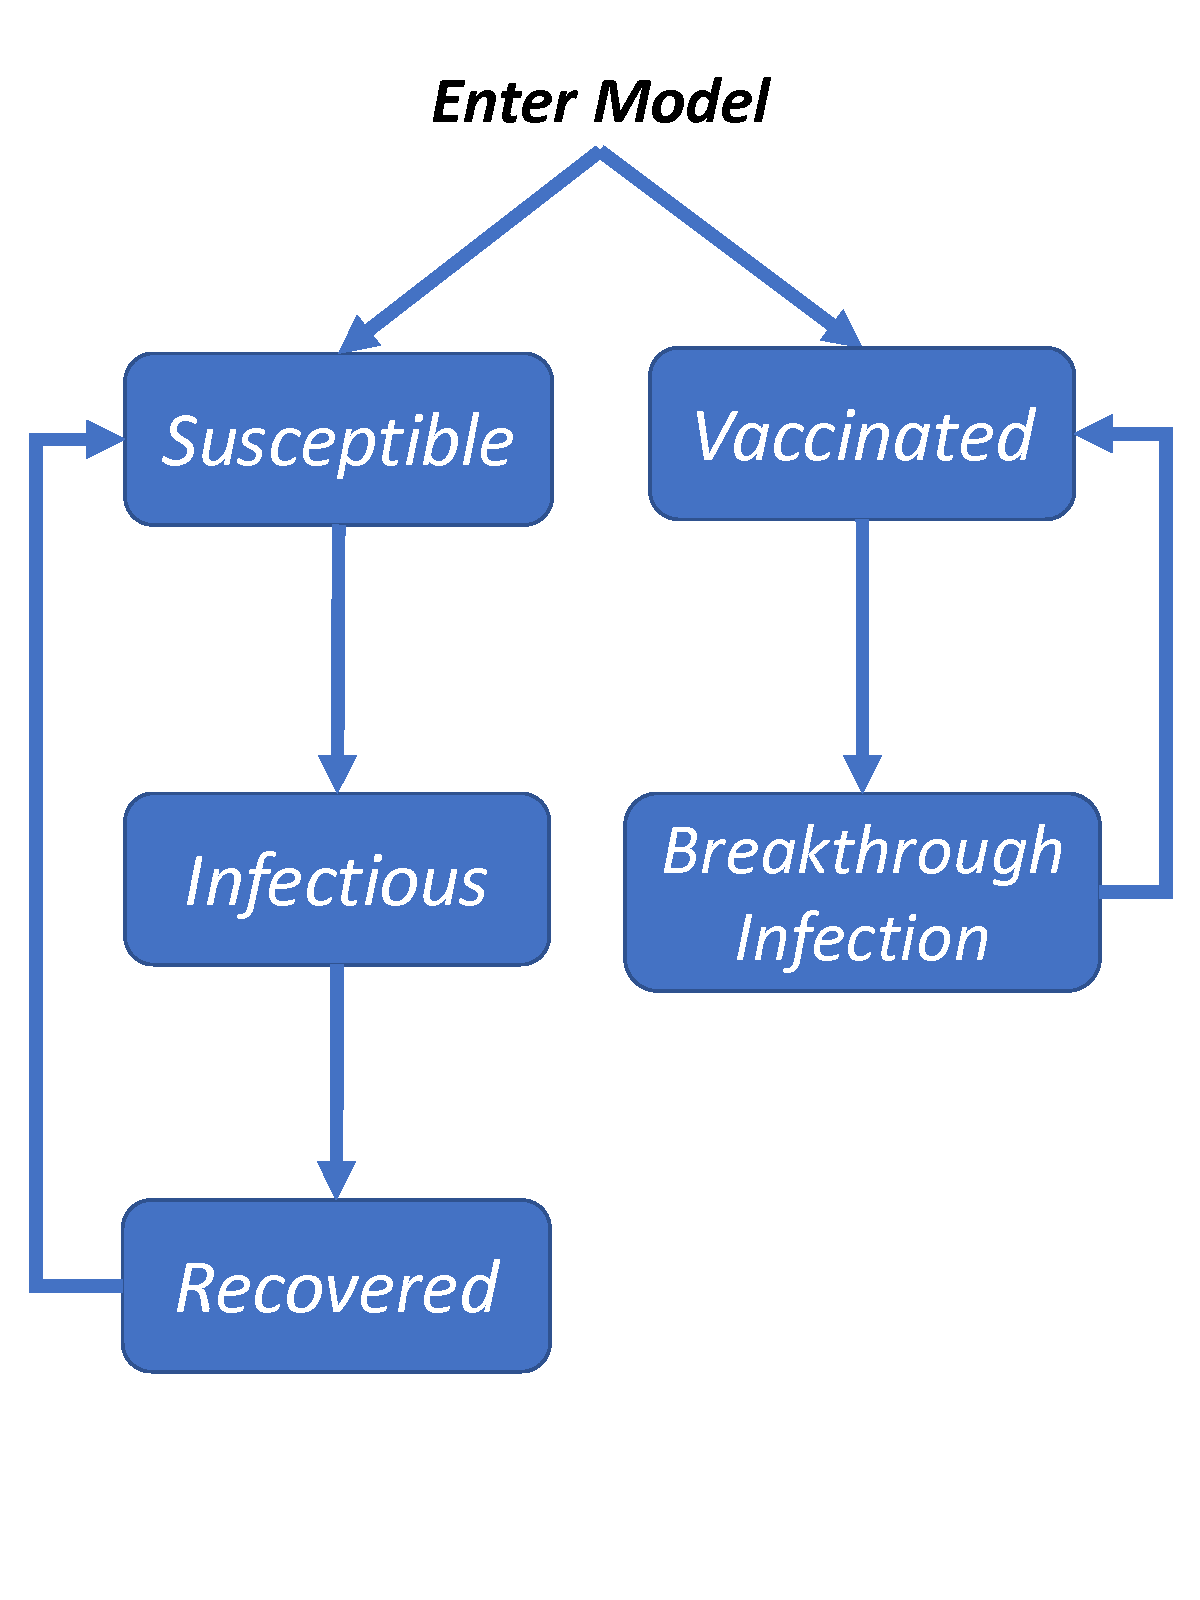
\includegraphics[trim ={0 3cm 0 0}, clip, width=0.7\textwidth]{good_model_flow}
            \caption{\scriptsize{Based on Hughes, et al. 2002}}
        \end{figure}
    \end{column}
    \begin{column}{0.5\textwidth}
    \pause
    \emph{Structure}
    \begin{itemize}
        \pause
        \item Three models: heterosexual only, multiple sexual identities, and averaged behavior
        \pause
        \item UK adults, 20-34 years old
        \pause
        \item 2 sexes (male, female)
        \pause
        \item 3 sexual identities (multiSexID only): heterosexual, gay/lesbian, bisexual
        \pause 
        \item 2 sexual activities (high/low)
        \pause
        \item Single type: HPV16
        \pause
        \item Sexual behavior data from National Survey on Sexual Attitudes and Lifestyles, 2010-2012
    \end{itemize}
    \end{column}
    \end{columns}
\end{frame}

\begin{frame}{Model Details}
    \begin{columns}[T]
    \begin{column}{0.5\textwidth}
        \begin{figure}
            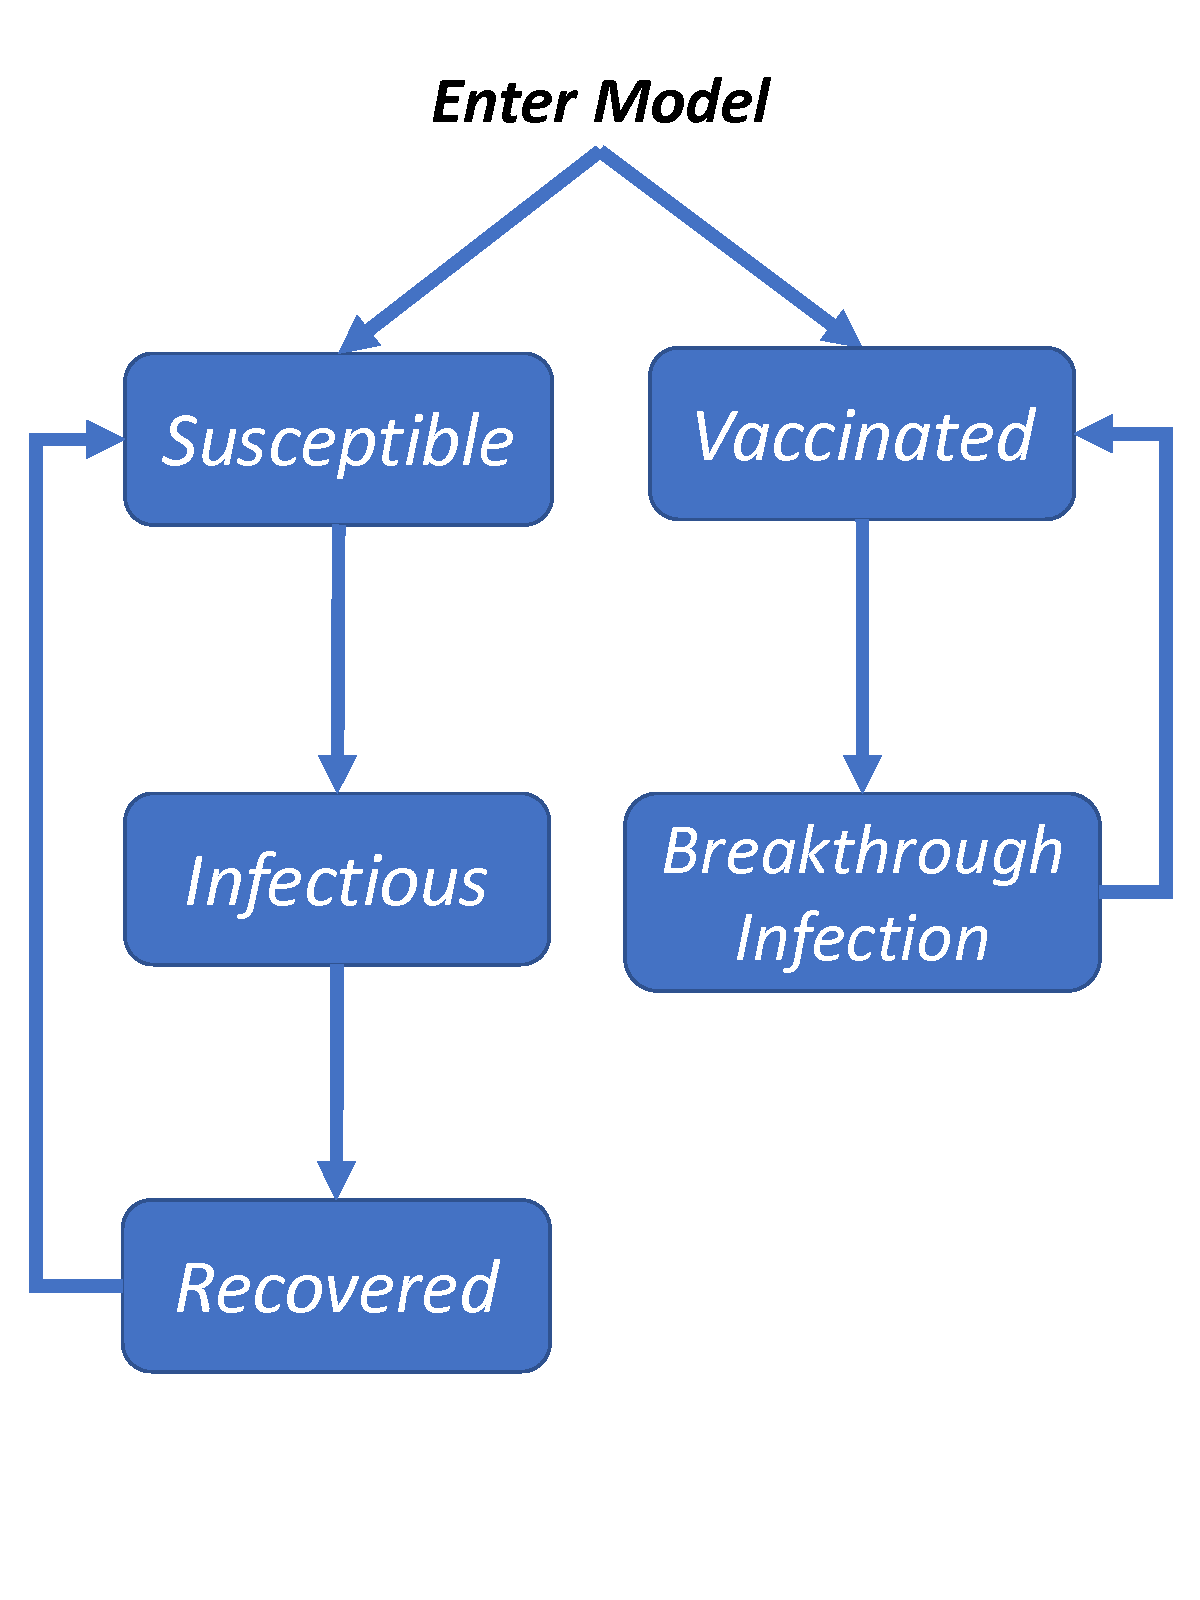
\includegraphics[trim ={0 3cm 0 0}, clip, width=0.7\textwidth]{good_model_flow}
            \caption{\scriptsize{Based on Hughes, et al. 2002}}
        \end{figure}
    \end{column}
    \begin{column}{0.5\textwidth}
    \emph{Calibration}
    \pause
        \begin{itemize}
        \item Bayesian calibration to pre-vaccination male  and female HPV16 prevalence
        \end{itemize}
    \pause
    \medskip
    \emph{Intervention}
    \pause
    \begin{itemize}
        \item Assuming 70\% female vaccination coverage, introduce 70\% male coverage
    \end{itemize}
    \medskip
    \pause
    \emph{Outcome}
    \pause
    \begin{itemize}
        \item Number of infections prevented by male vaccination,  over 20 years
    \end{itemize}
    \end{column}
    \end{columns}
\end{frame}

\begin{frame}{Contact Between Groups: Heterosexual} 
    \vspace{2cm}
    \centering
    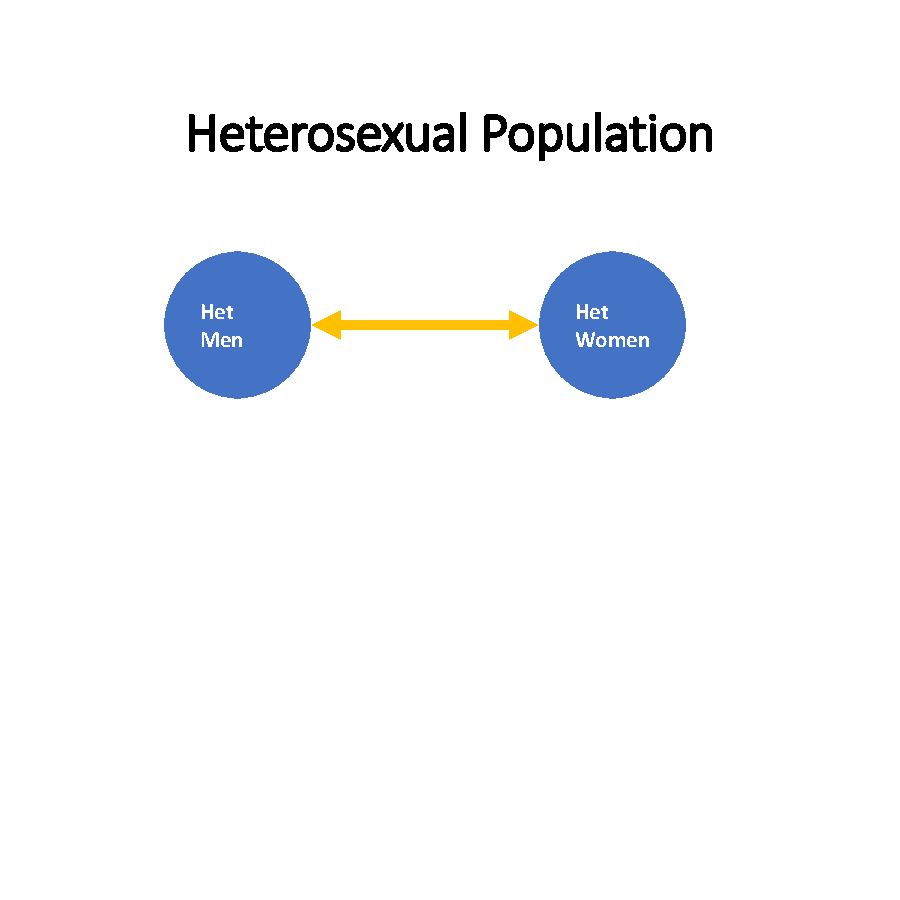
\includegraphics[trim = {0 0 0 3cm}, clip, width=0.7\textwidth]{het_population.pdf}
\end{frame}

\begin{frame}{Contact Between Groups: Heterosexual}
    \centering
    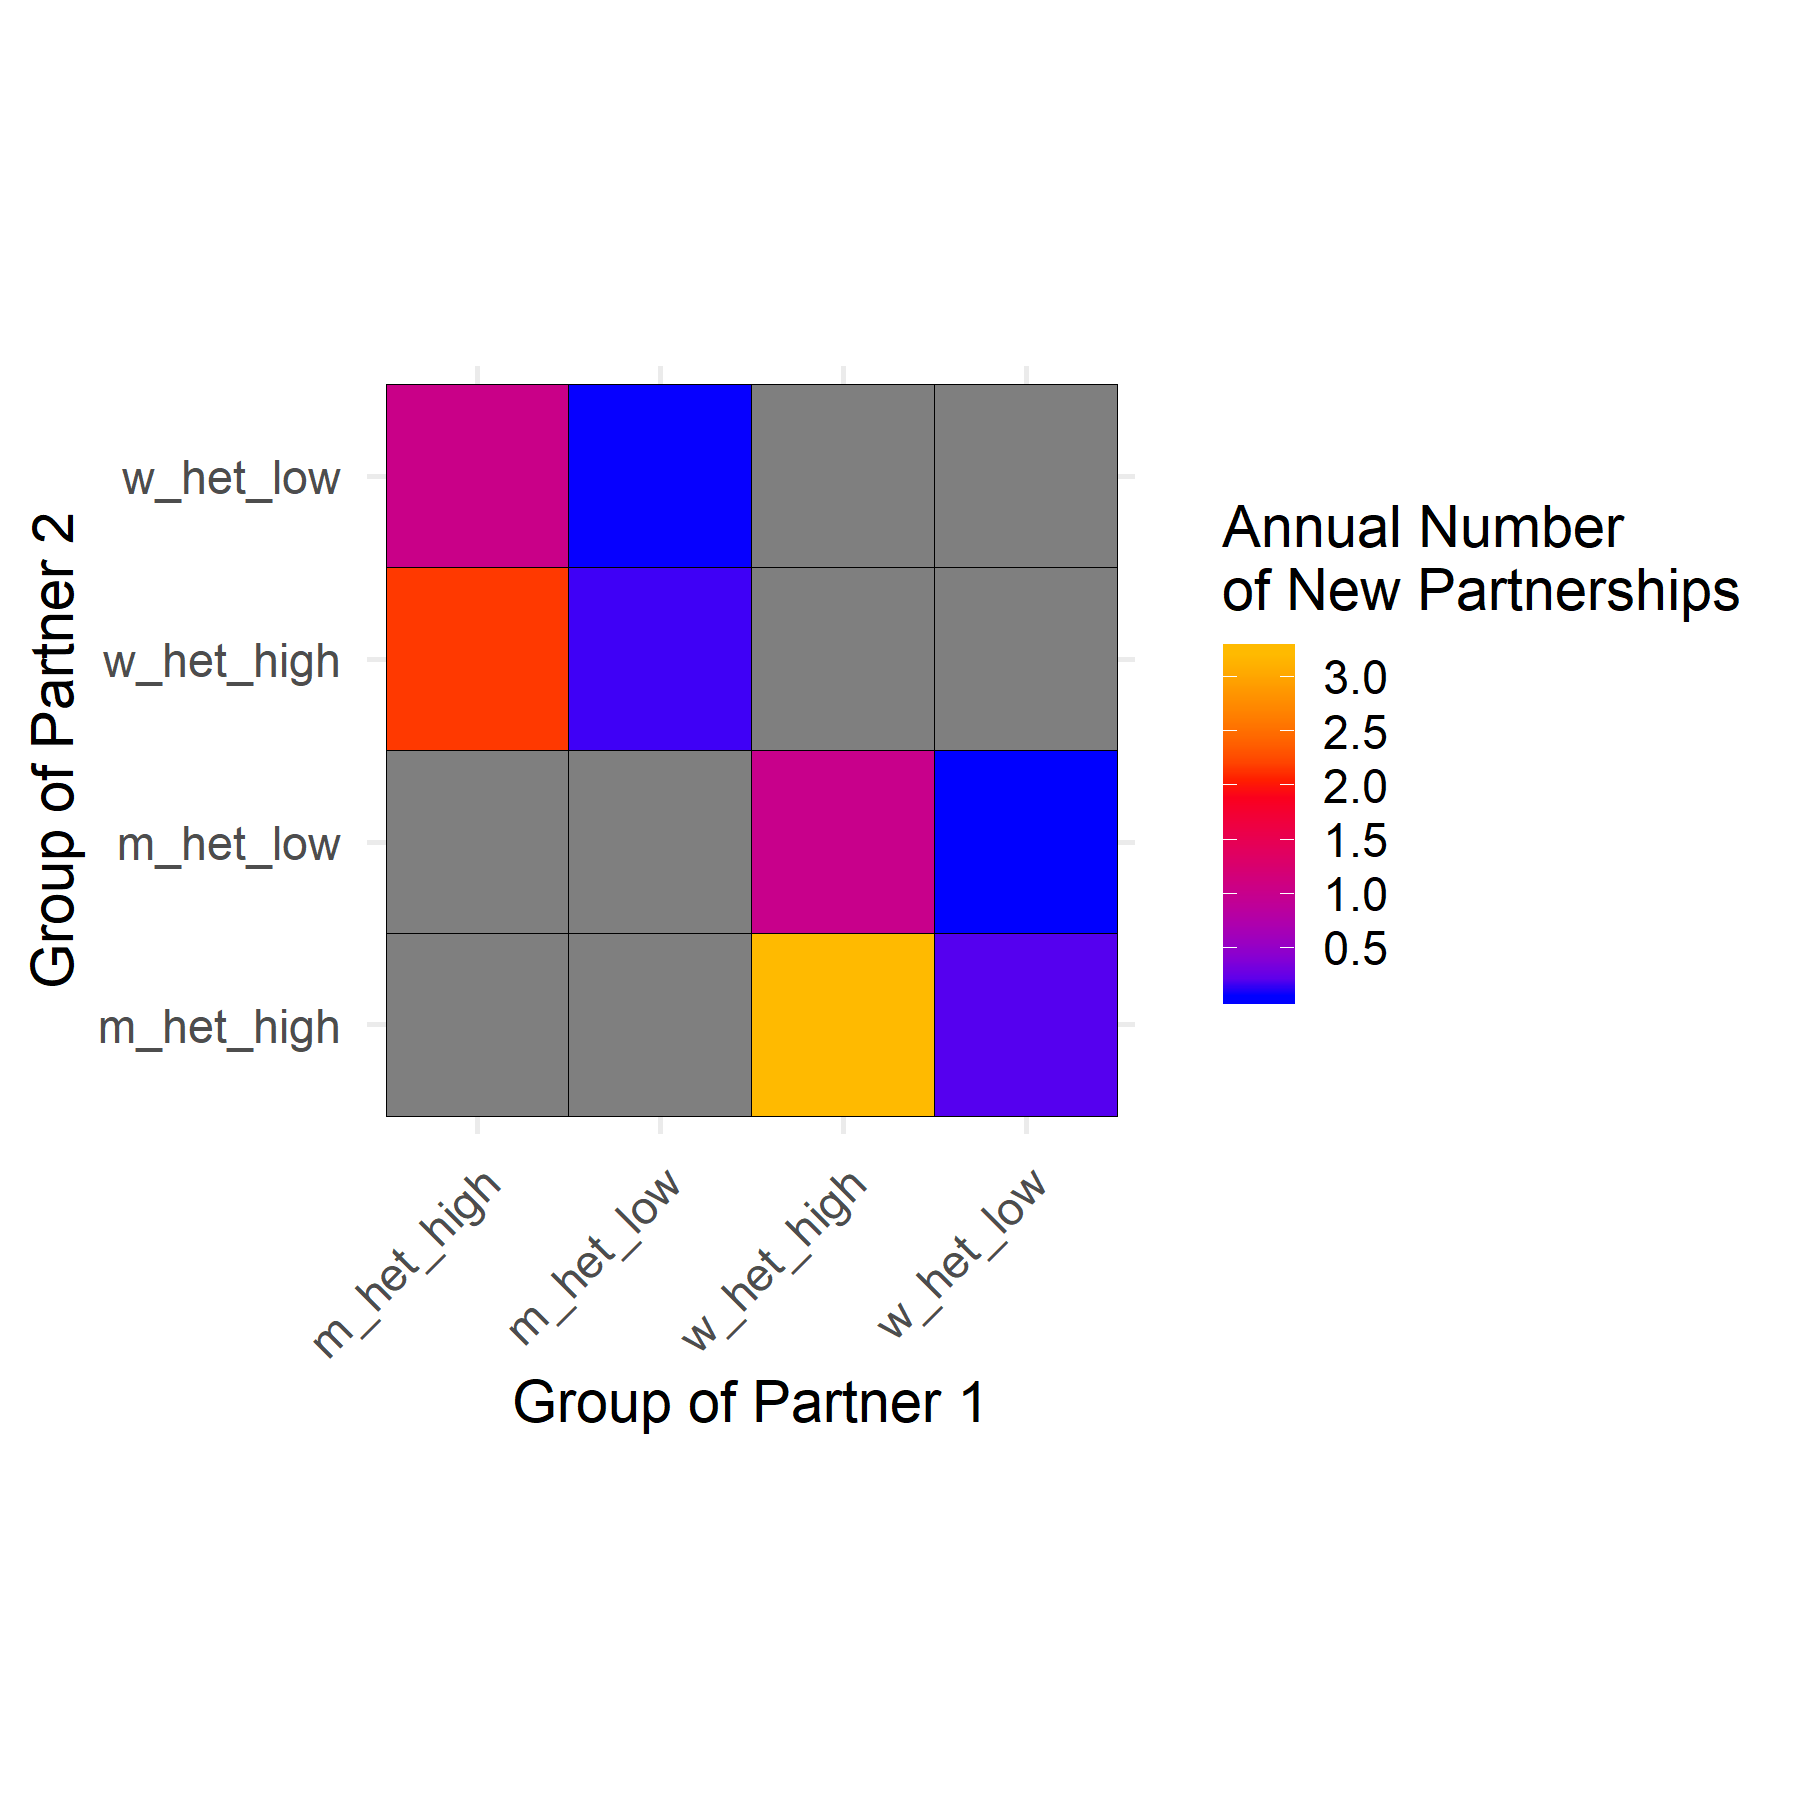
\includegraphics[trim = {0 0 0 2cm}, clip,width=0.7\textwidth]{het_only}
\end{frame}

\begin{frame}{Contact Between Groups: Multiple Sex ID}
    \centering
    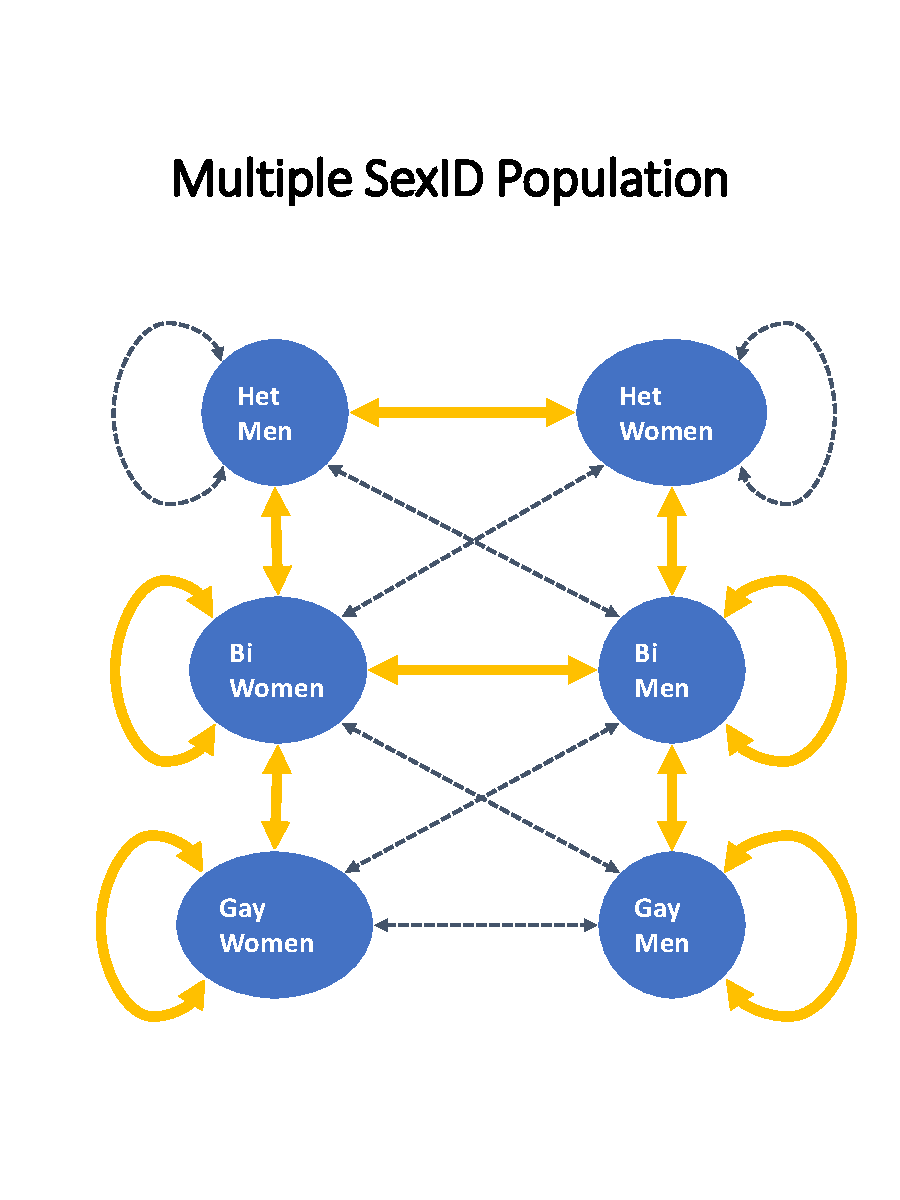
\includegraphics[trim ={0 0 0 5cm}, clip, width=0.6\textwidth]{mult_sexid_population}
\end{frame}

\begin{frame}{Contact Between Groups: Multiple Sex ID}
    \centering
    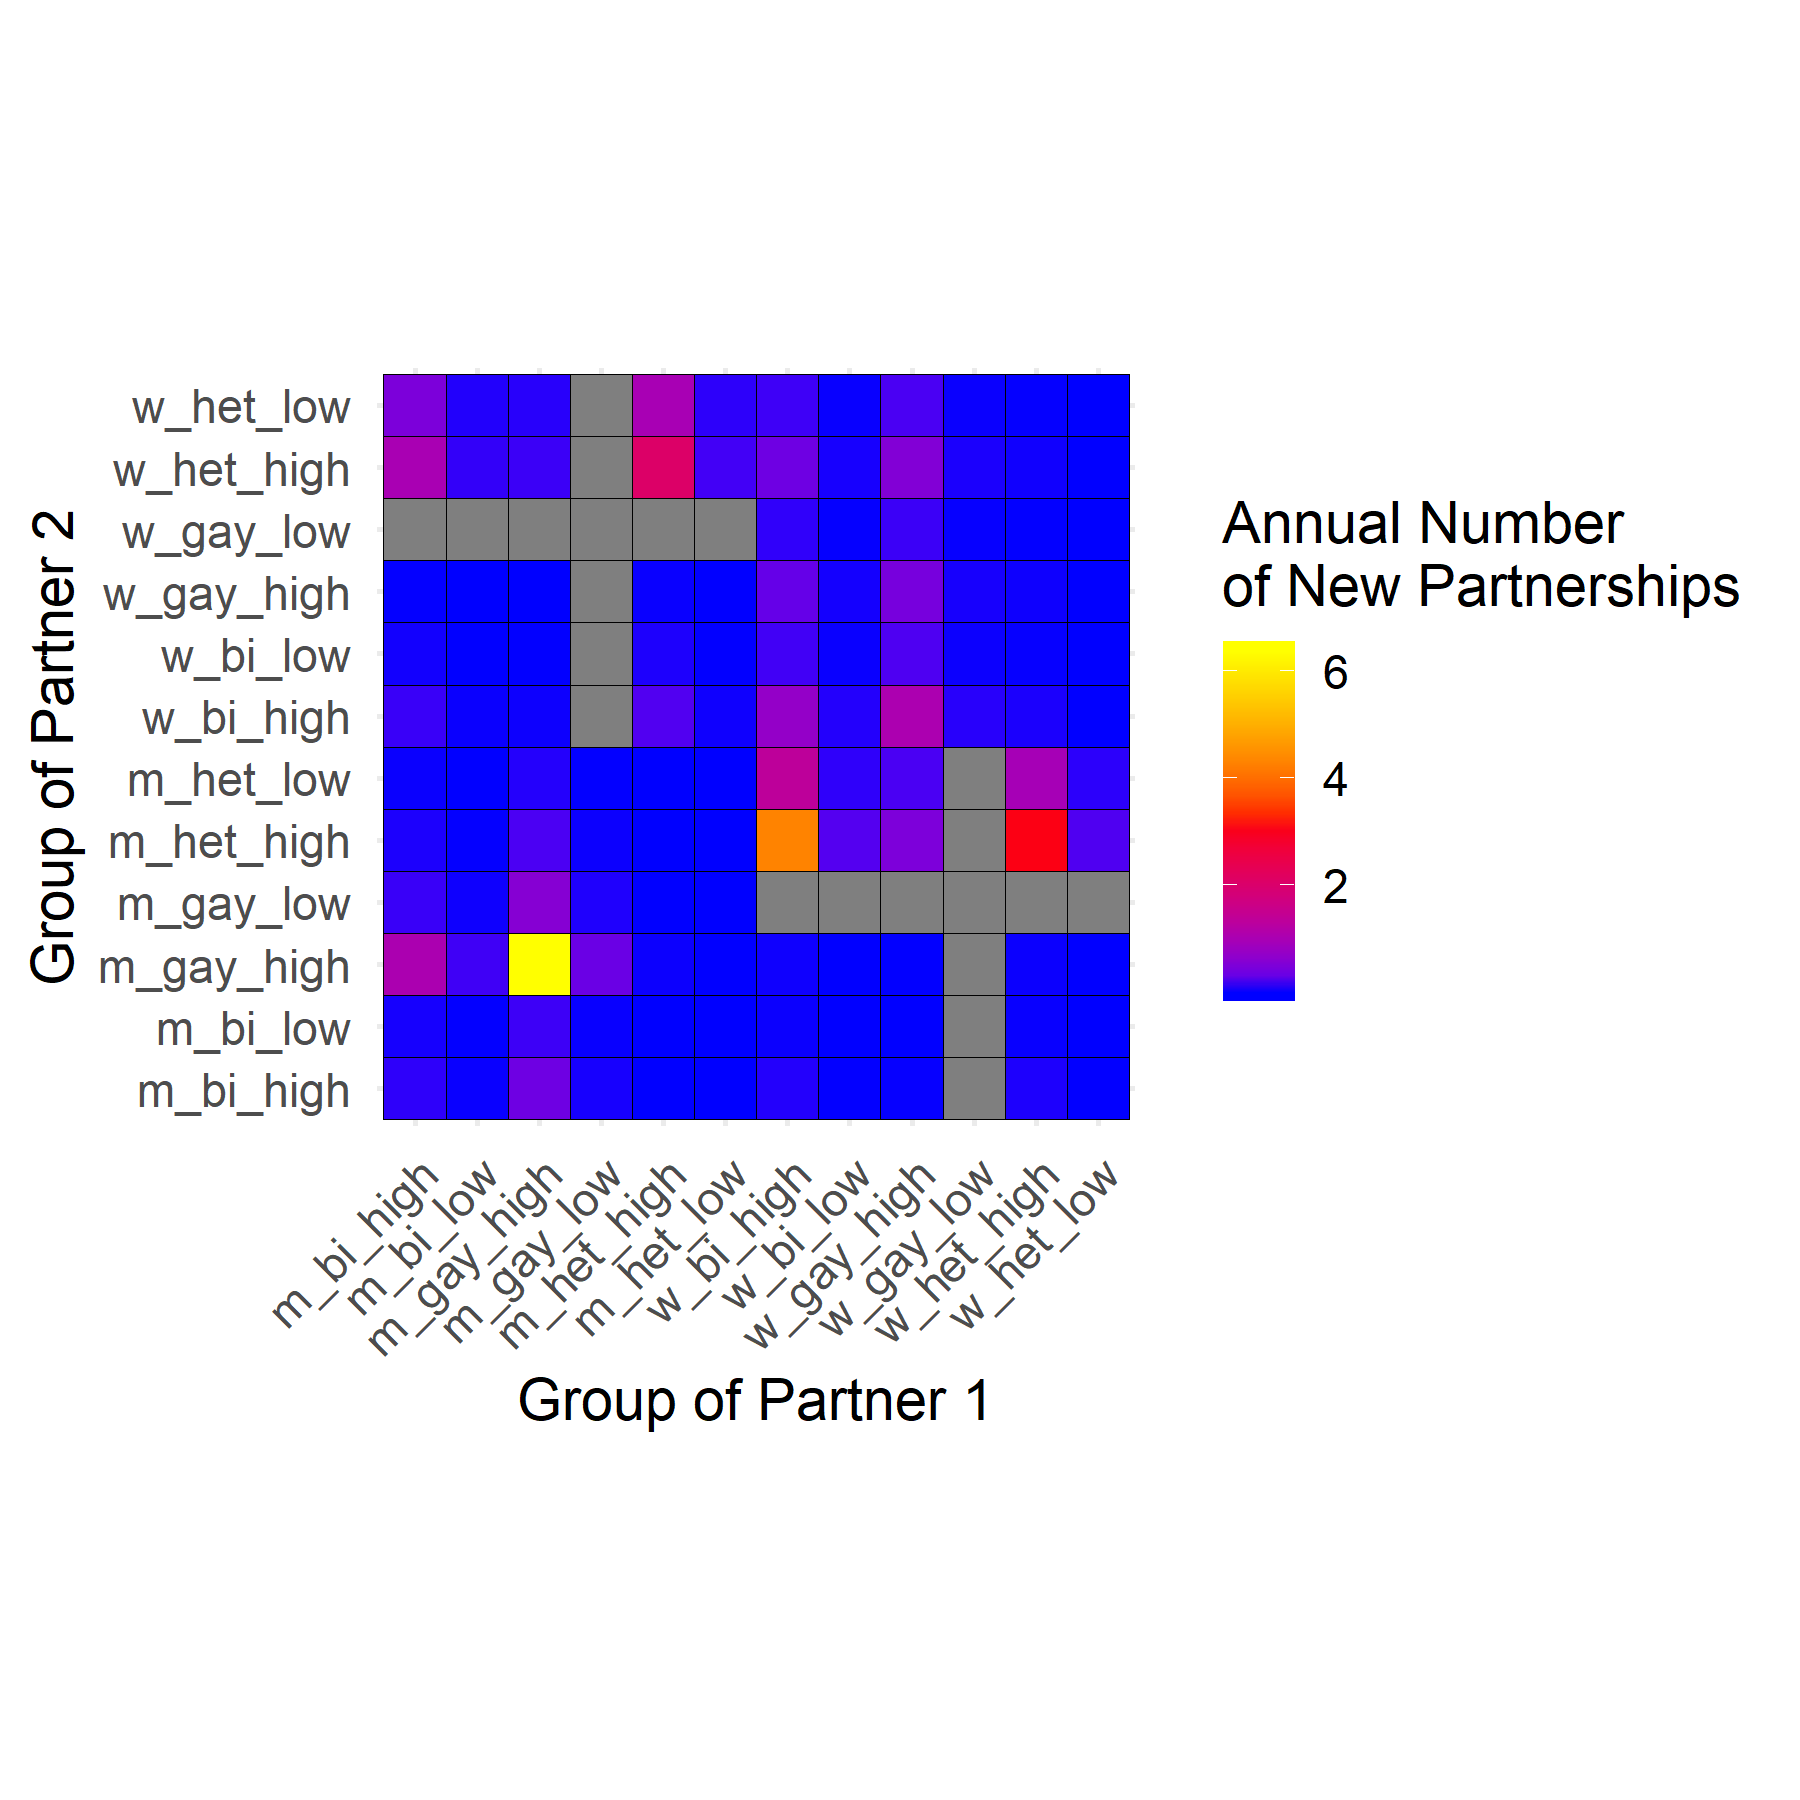
\includegraphics[trim = {0 0 0 2cm}, clip, width=0.7\textwidth]{all_sexid}
\end{frame}

\begin{frame}{Contact Between Groups: Averaged Multiple Sex ID}
    \centering
    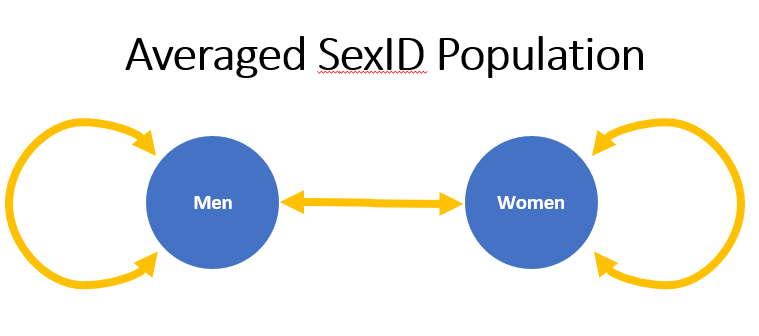
\includegraphics[width=0.7\textwidth]{averaged_sexid}
\end{frame}

\begin{frame}{Contact Between Groups: Averaged Multiple Sex ID}
    \centering
    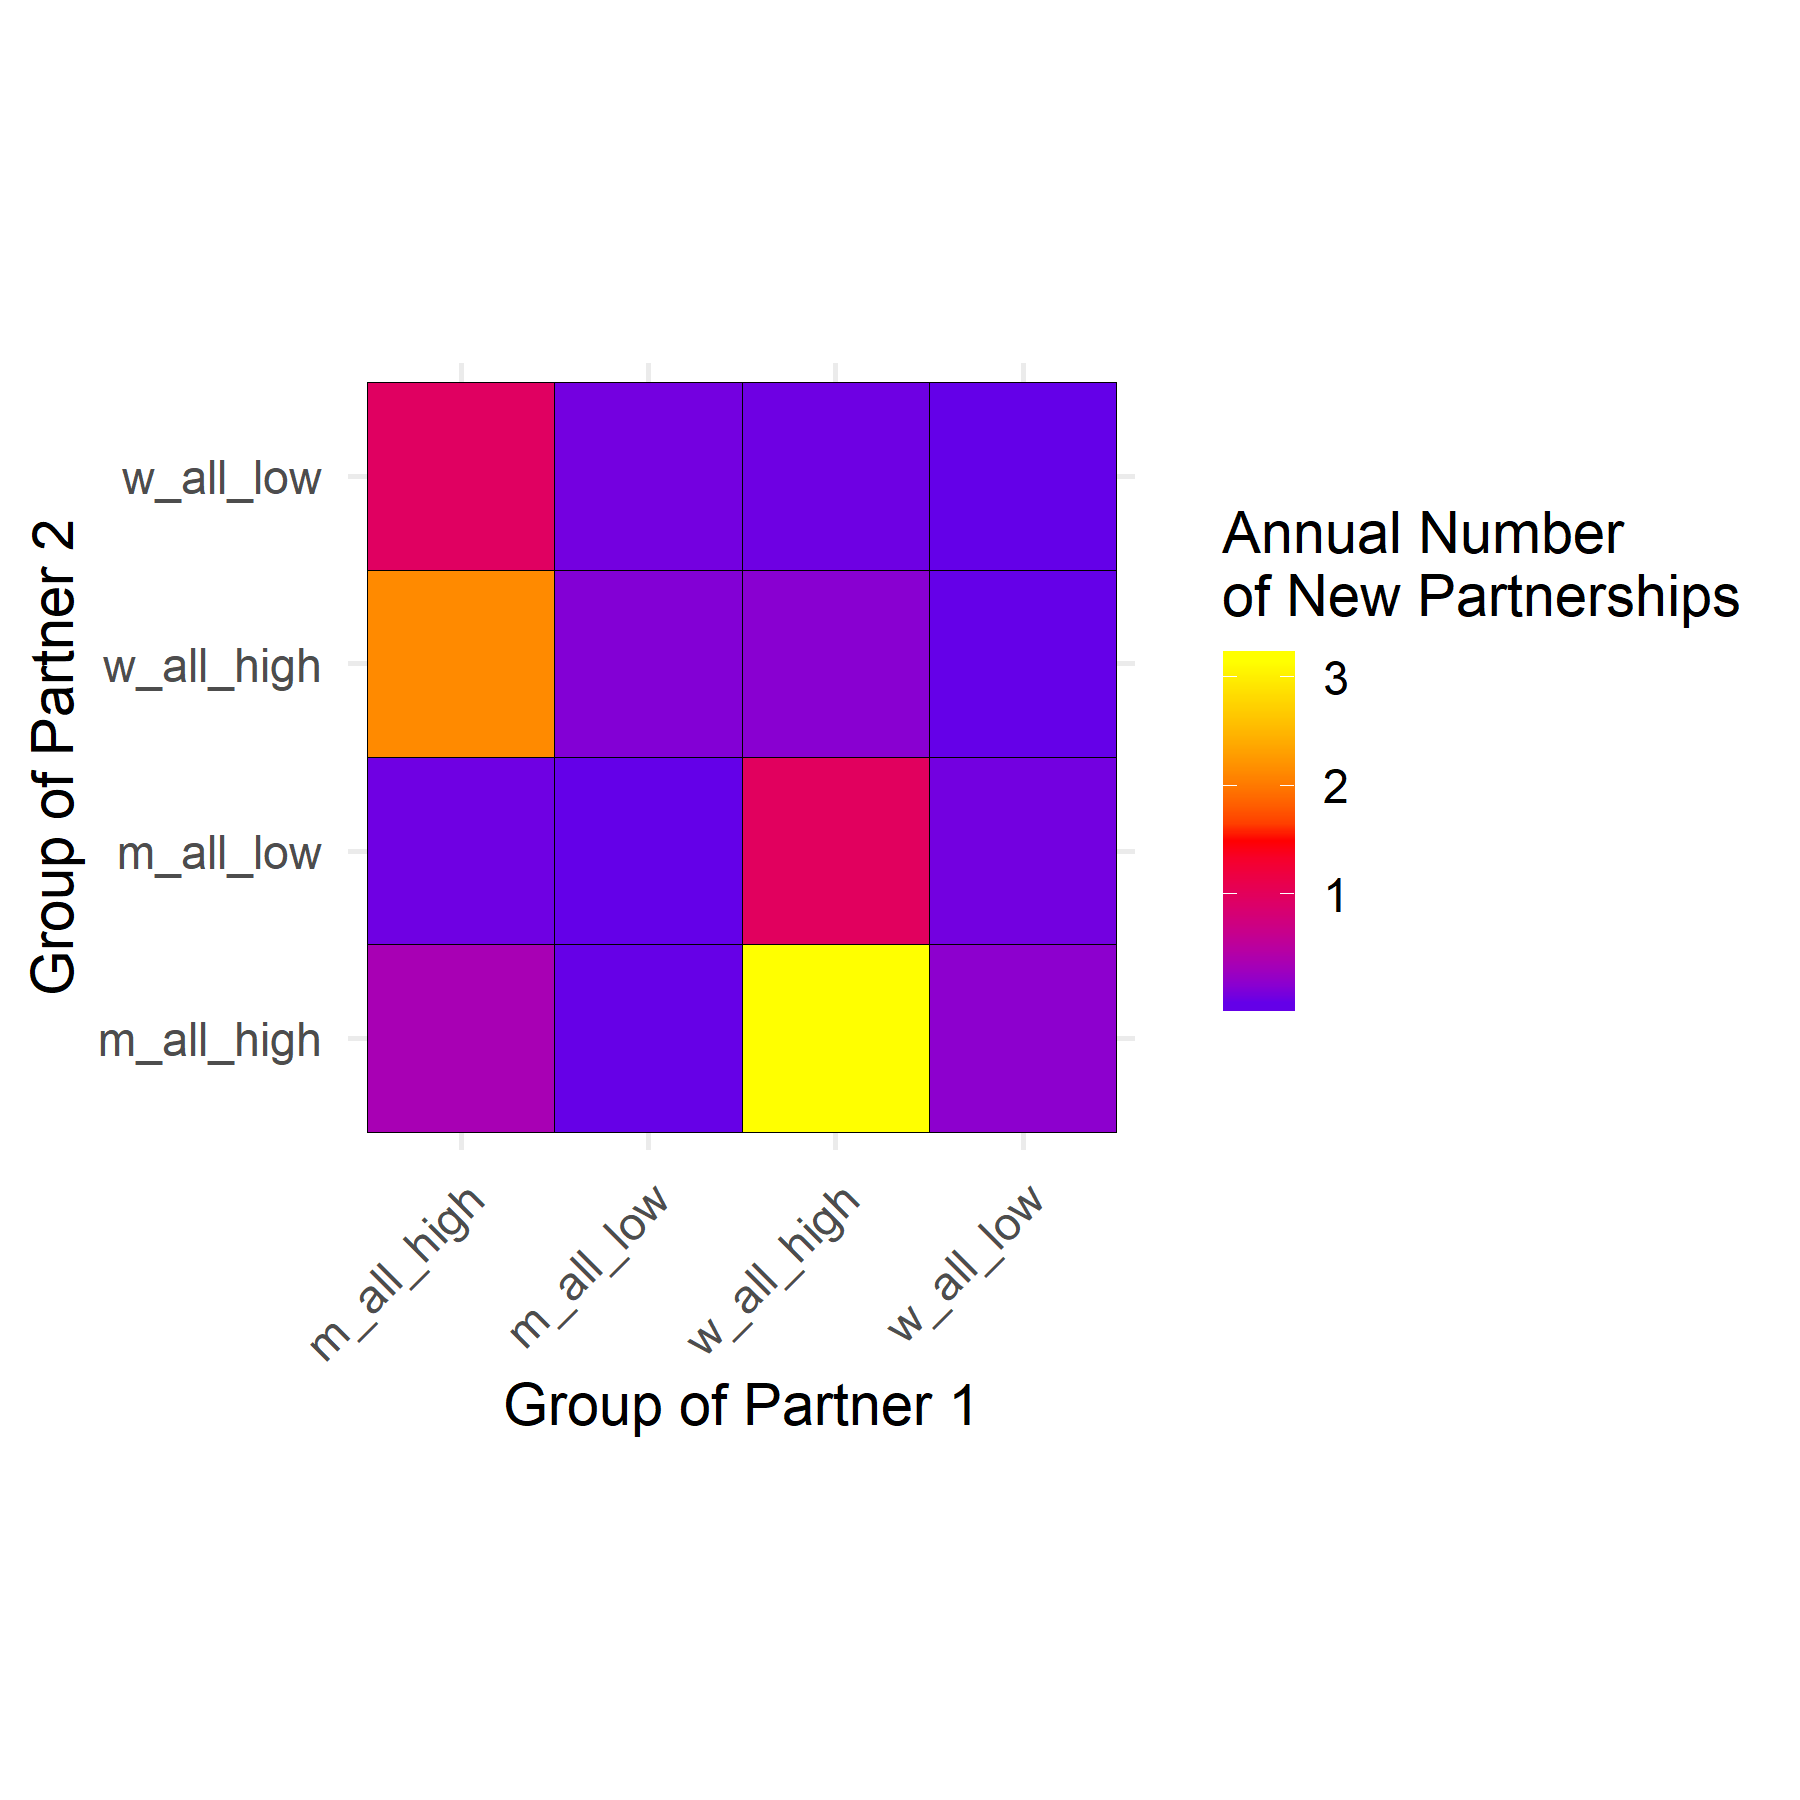
\includegraphics[trim ={0 0 0 2cm}, clip, width=0.7\textwidth]{all_tog}
\end{frame}

\begin{frame}{Results}
    \centering
    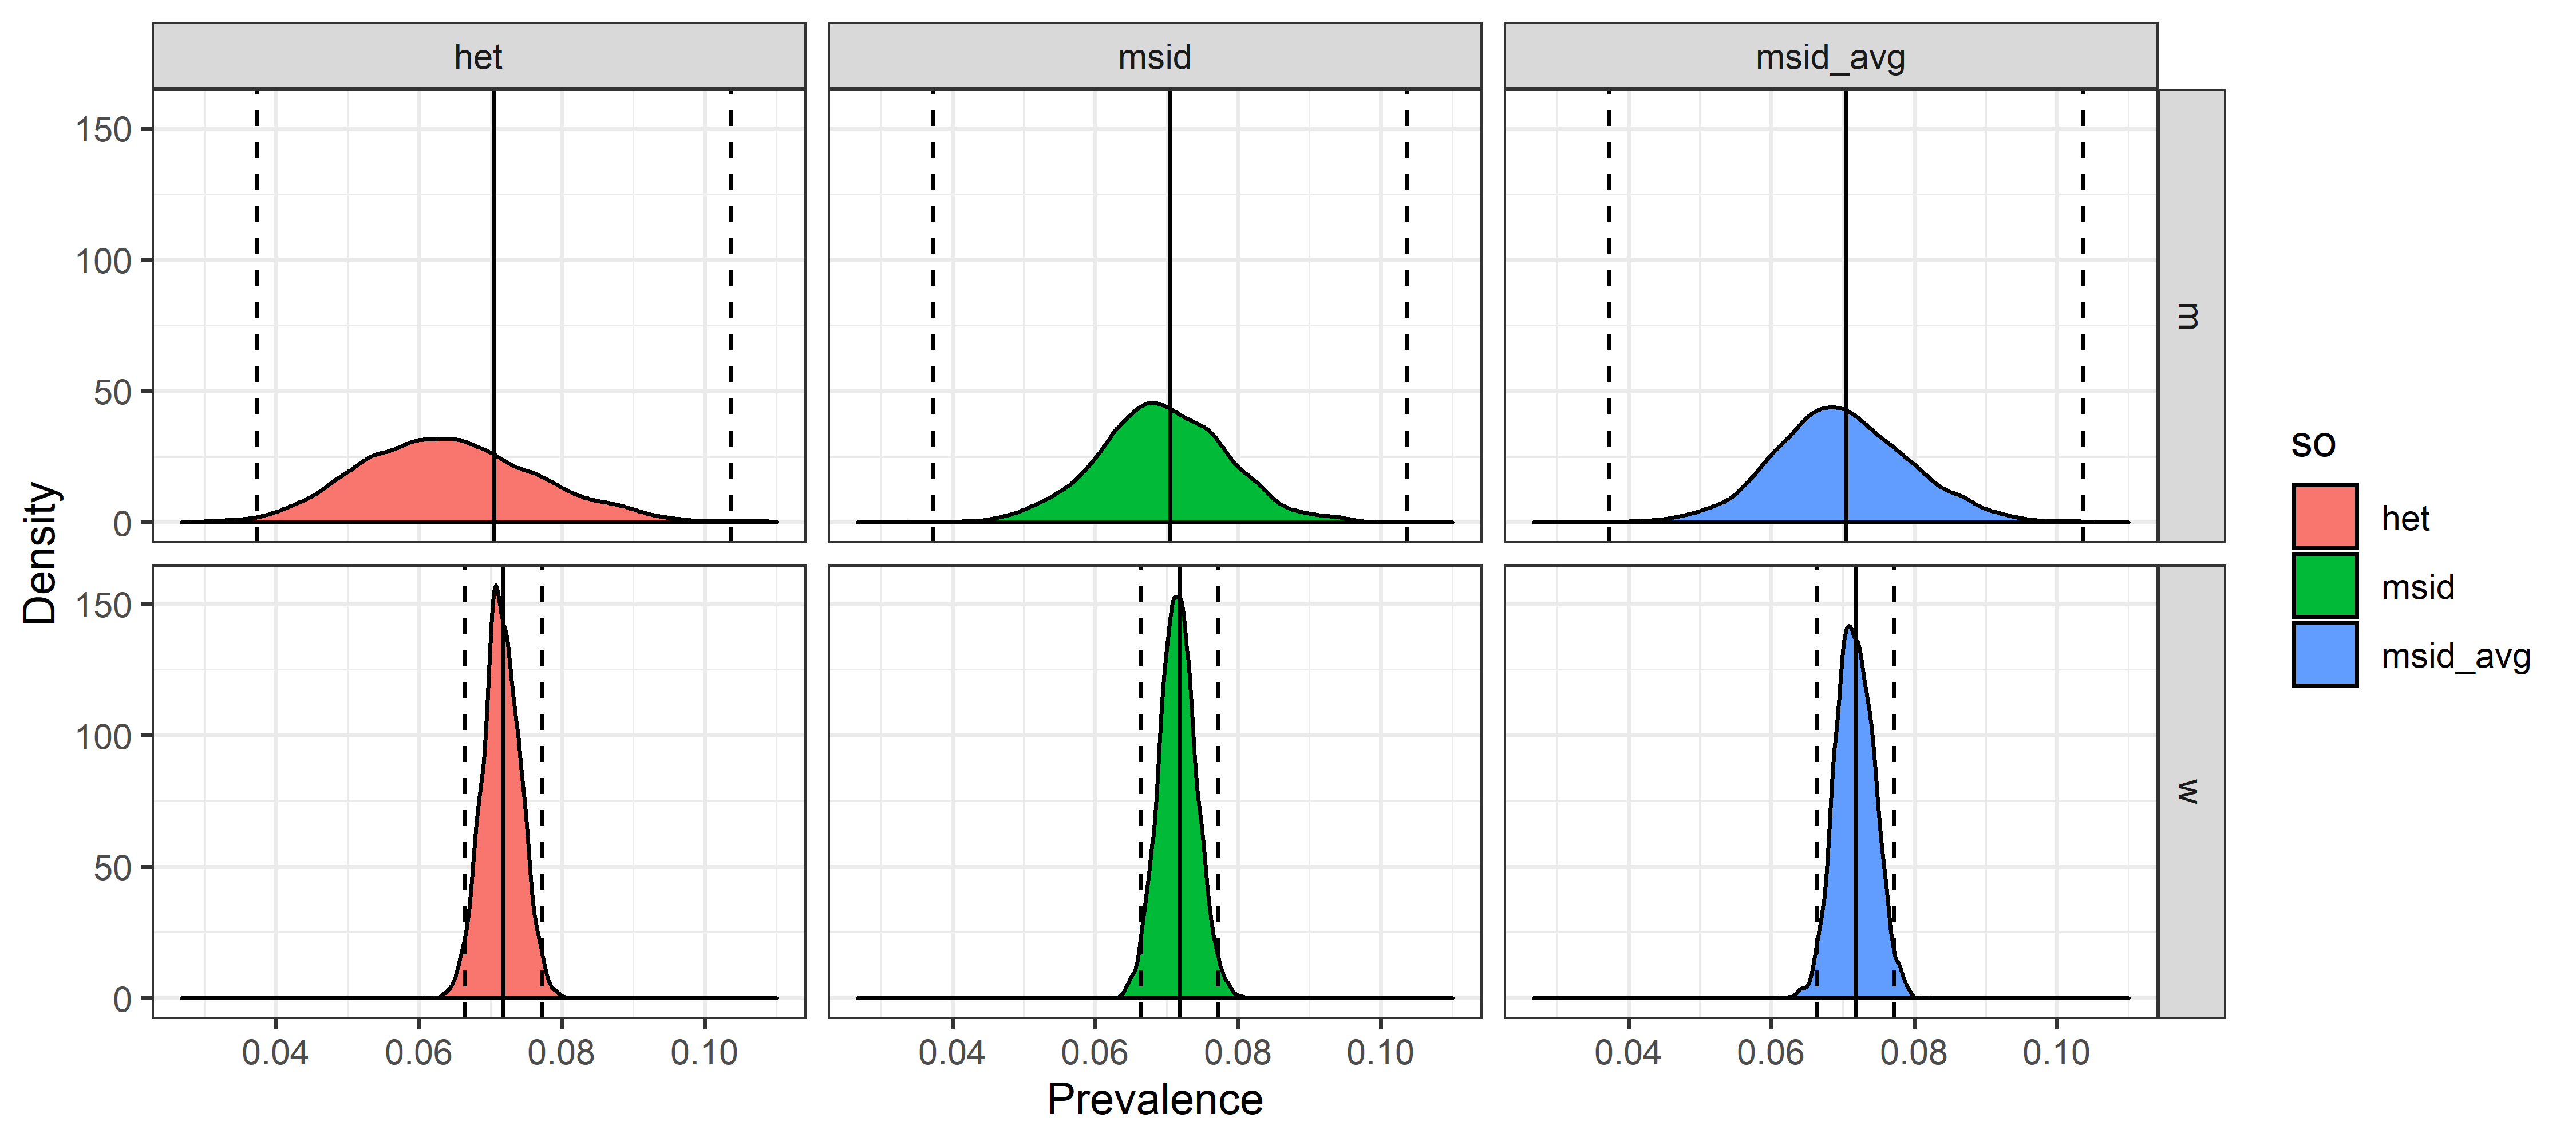
\includegraphics[width=1\textwidth]{calib_results_03_23_2020_v2}
\end{frame}

\begin{frame}{Results}
    \begin{center}
        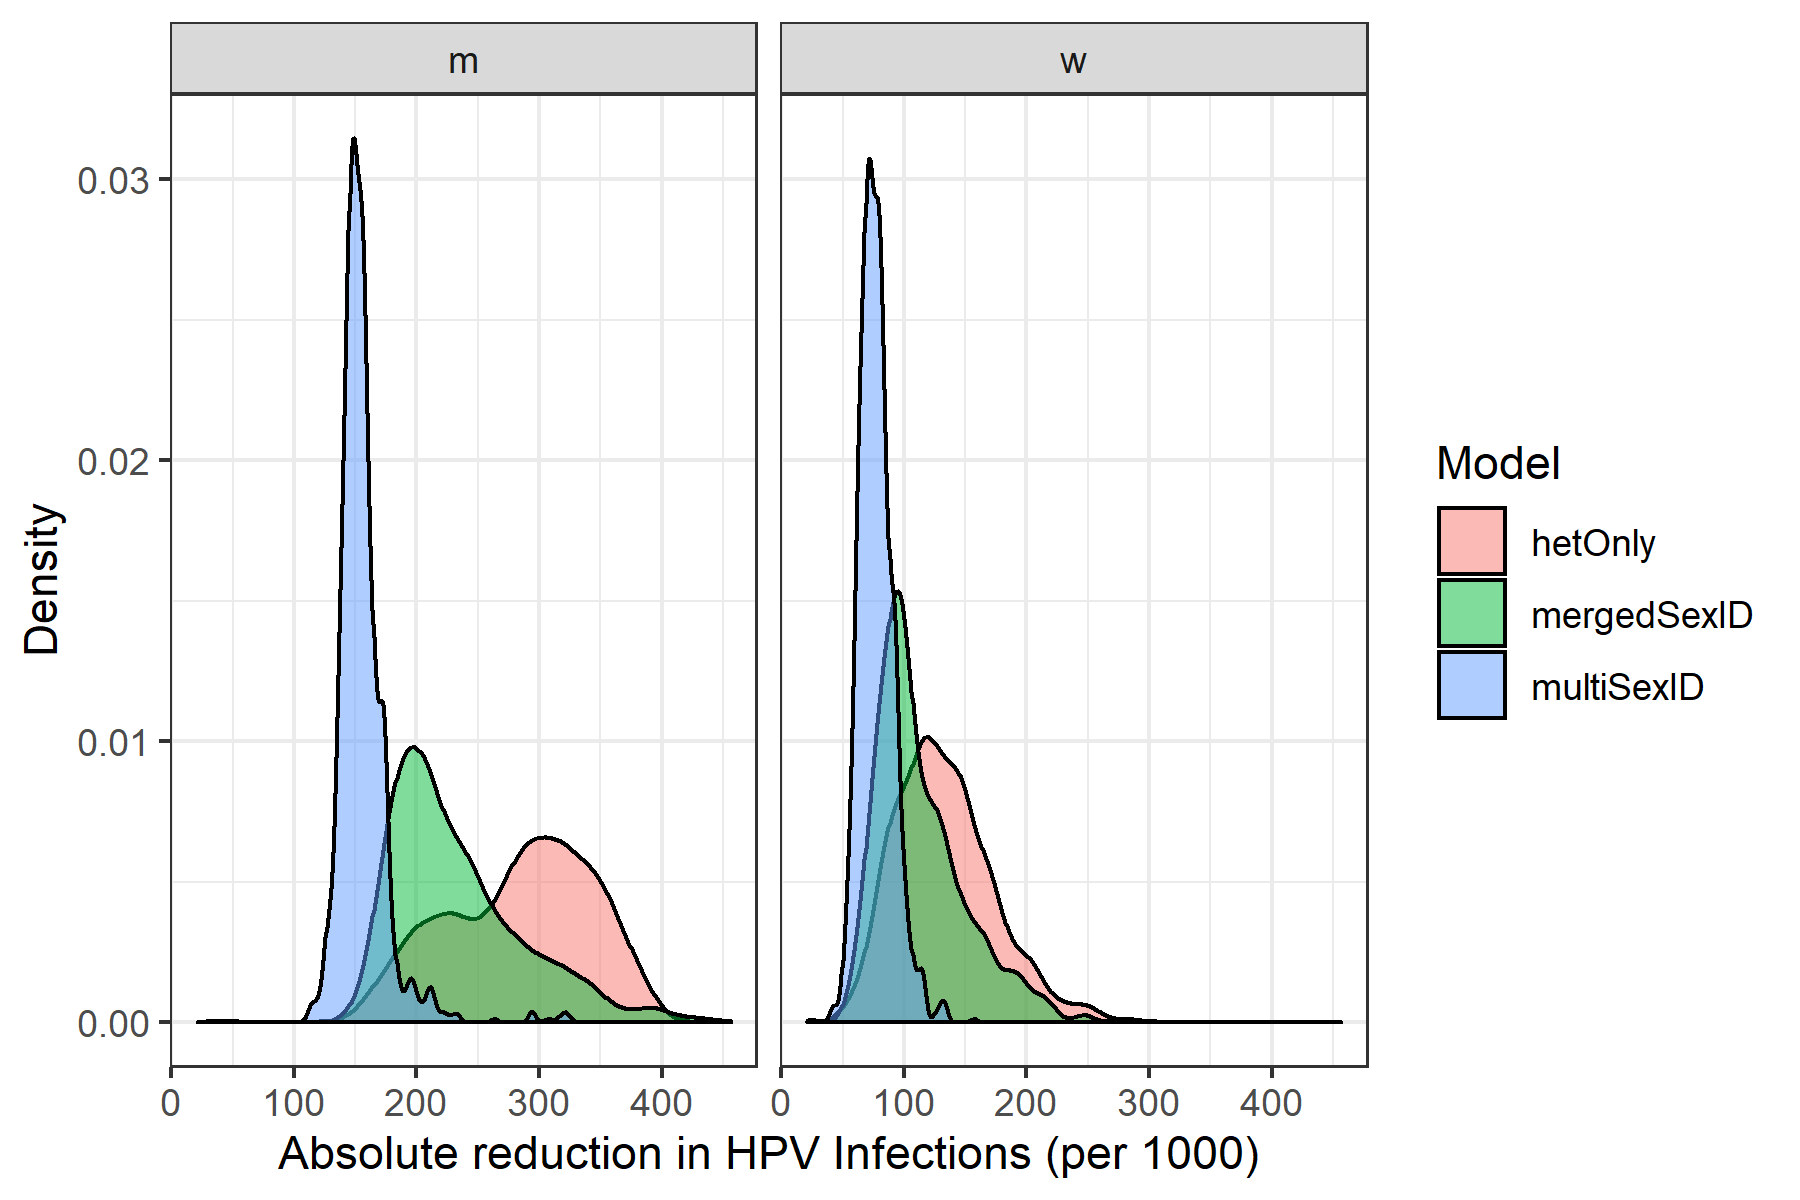
\includegraphics[width=0.8\textwidth]{absolute_50}
    \end{center}
\end{frame}


\begin{frame}{Conclusions}
    \begin{itemize}
            \pause
            \item A model with only heterosexual sex predicted a much greater reduction in infections due to male HPV vaccination than an identical model multiple sexual identities.
            \pause
            \item Much of this may be due to differences in the calibrated models.
            \pause
            \item The omission of multiple sexual identities may affect cost-effectiveness estimates for male HPV vaccination.
            \pause
            \item Including multiple sexual orientations is more representative of true population, and provides a `seat at the table' for those who do not identify as heterosexual
            \pause
            \item As in other study types, modeling studies should strive to ensure that their model population is as representative of the target population as possible, to facilitate valid generalization of results
    \end{itemize}
\end{frame}

\begin{frame}{Future Directions}
	\begin{itemize}
      	     \item Fix the epidemiological parameters to be the same across models and re-calibrate \pause
            \item Expand model to include age and further disease states. \pause
            \item Compare cost-effectiveness estimates of different vaccination strategies under each model
	\end{itemize}
\end{frame}

%\begin{frame}{References}
%\nocite{*}
%\printbibliography
%\end{frame}

\begin{frame}{Thank you!}
\centering
\huge
Any Questions?
\end{frame}



\end{document}
